% =====================================================================
%  Paper_Explained_Simple.tex -- plain-language walkthrough of the
%  IEEE paper (sc_two_column.pdf) for the project team.
%  Updated after training (results from 16-17 Oct 2026).
%  Build: tectonic Paper_Explained_Simple.tex
% =====================================================================
\documentclass[11pt,a4paper]{article}
% =====================================================================
%  report_preamble.tex -- shared preamble for the stand-alone
%  Datasets and Algorithms reports (article class, A4).
% =====================================================================
\usepackage[T1]{fontenc}
\usepackage[utf8]{inputenc}
\usepackage{mathptmx}
\usepackage[a4paper,margin=2cm]{geometry}
\usepackage{amsmath,amssymb}
\usepackage{graphicx,xcolor}
\usepackage{tikz,pgfplots}
\pgfplotsset{compat=1.18}
\usetikzlibrary{positioning,arrows.meta,calc}
\usepackage{booktabs,array,multirow,tabularx,longtable}
\usepackage{pifont}
\providecommand{\checkmark}{\ding{51}}
\usepackage{enumitem}
\setlist{itemsep=1pt,topsep=3pt,parsep=0pt}
\usepackage[font=small,labelfont=bf]{caption}
\usepackage{float}
\usepackage{cite}
\usepackage{url}
\usepackage[colorlinks=true,linkcolor=hcBlue,citecolor=hcBlue,urlcolor=hcTeal]{hyperref}
\usepackage{titlesec}
\titleformat{\section}{\large\bfseries\color{hcBlue}}{\thesection}{0.6em}{}
\titleformat{\subsection}{\normalsize\bfseries}{\thesubsection}{0.6em}{}
\setlength{\parskip}{3pt}

% ---- Palette (colour-blind friendly) ----------------------------------
\definecolor{hcBlue}{HTML}{2166AC}
\definecolor{hcTeal}{HTML}{1B9E77}
\definecolor{hcOrange}{HTML}{D95F02}
\definecolor{hcPurple}{HTML}{7570B3}
\definecolor{hcRed}{HTML}{B2182B}
\definecolor{hcGray}{HTML}{6E6E6E}
\definecolor{boxBg}{HTML}{EEF3FA}

\pgfplotsset{
  hcaxis/.style={
    tick align=outside, tick pos=left, grid=major,
    major grid style={line width=0.2pt,draw=gray!30},
    axis line style={draw=gray!55},
    label style={font=\footnotesize},
    tick label style={font=\scriptsize},
    legend style={font=\scriptsize,draw=gray!40,fill=white,rounded corners=1pt},
    every node near coord/.append style={font=\tiny},
  }
}

\newcolumntype{L}[1]{>{\raggedright\arraybackslash}p{#1}}
\newcolumntype{Y}{>{\raggedright\arraybackslash}X}

% Highlight box for key take-aways
\newcommand{\keybox}[1]{%
  \par\smallskip\noindent\colorbox{boxBg}{\parbox{\dimexpr\linewidth-2\fboxsep}{\small #1}}\par\smallskip}

\setlength{\parindent}{0pt}

% "In simple words" box and "Where in the paper" tag
\newcommand{\simple}[1]{\keybox{\textbf{In simple words:} #1}}
\newcommand{\where}[1]{{\small\color{hcGray}\textit{Where in the paper: #1}}\par\smallskip}

\title{\color{hcBlue}\bfseries Our IEEE Paper Explained Simply\\[4pt]
\large ``Skin Cancer Detection Using Deep Learning: A Comparative Analysis\\
and a Multi-Model CNN--Transformer Ensemble with External Validation''}
\author{Team guide --- read this with \texttt{sc\_two\_column.pdf} open next to it}
\date{}

\begin{document}
\maketitle
\vspace{-6mm}
\tableofcontents
\newpage

% =====================================================================
\section{The Whole Paper in One Minute}
\begin{itemize}
  \item \textbf{Topic:} using AI to look at a photo of a skin spot and
        say whether it may be skin cancer.
  \item \textbf{Problem we found:} many papers claim 95--99\% accuracy,
        but these numbers are often too good to be true. The same photo
        (or the same mole) appears in both training and testing, models
        are never tested on photos from other hospitals, and they work
        worse on dark skin.
  \item \textbf{What we did:}
  \begin{enumerate}
    \item Read and summarized 40+ research papers (literature review).
    \item Studied 12 public datasets and chose the best two.
    \item Designed our system (proposed methodology) and an honest
          testing plan (experimental design).
    \item \textbf{Trained 3 models} --- EfficientNetV2-S and ConvNeXt-T
          (CNNs) and Swin-T (transformer) --- on ISIC 2019 and
          \textbf{combined their votes} (our USP).
    \item Compared everything with 11 kinds of published algorithms
          (comparative analysis).
  \end{enumerate}
  \item \textbf{Our main result:} on 3{,}596 test images the combined model
        reached \textbf{77.95\% accuracy}, \textbf{62.99\% balanced accuracy},
        AUC \textbf{0.950}, and caught \textbf{95.4\%} of cancers --- better
        than any single model or any pair of models.
  \item \textbf{Honest finding:} on phone photos from another country
        (PAD-UFES-20) accuracy fell to 37\%. \emph{How} and \emph{where} you
        test a model matters more than \emph{which} model you choose.
\end{itemize}

\simple{The paper says: ``Here is what everyone else has done, here is
what is still wrong, here is the best data, here is our 3-model system,
here are our real results, and here is how they compare with others.''}

\subsection*{How the sections connect}
\begin{center}
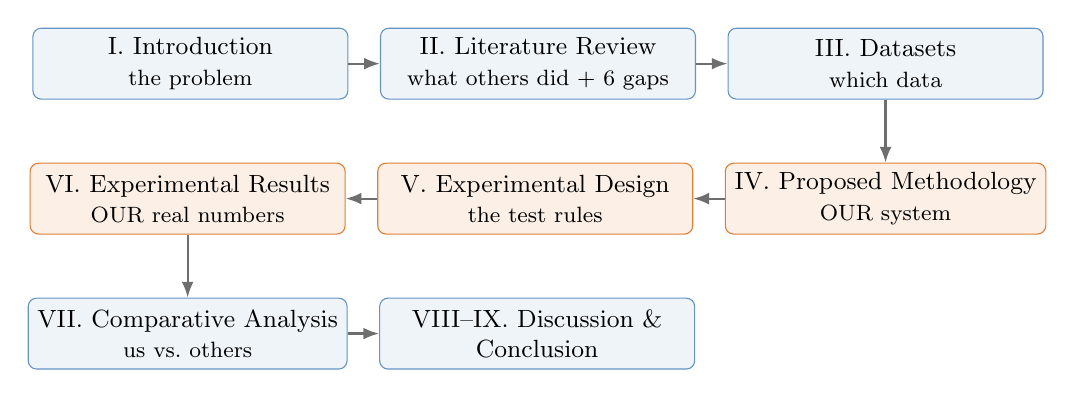
\begin{tikzpicture}[font=\small, node distance=4mm,
  b/.style={draw=hcBlue!70,fill=hcBlue!7,rounded corners=3pt,minimum width=40mm,minimum height=9mm,align=center},
  o/.style={draw=hcOrange!80,fill=hcOrange!10,rounded corners=3pt,minimum width=40mm,minimum height=9mm,align=center},
  fl/.style={-{Latex[length=2mm]},draw=hcGray,thick}]
\node[b] (i) {I. Introduction\\\footnotesize the problem};
\node[b,right=of i] (l) {II. Literature Review\\\footnotesize what others did + 6 gaps};
\node[b,right=of l] (d) {III. Datasets\\\footnotesize which data};
\node[o,below=8mm of d] (m) {IV. Proposed Methodology\\\footnotesize OUR system};
\node[o,left=of m] (e) {V. Experimental Design\\\footnotesize the test rules};
\node[o,left=of e] (r) {VI. Experimental Results\\\footnotesize OUR real numbers};
\node[b,below=8mm of r] (c) {VII. Comparative Analysis\\\footnotesize us vs.\ others};
\node[b,right=of c] (x) {VIII--IX. Discussion \&\\Conclusion};
\draw[fl] (i)--(l); \draw[fl] (l)--(d); \draw[fl] (d)--(m); \draw[fl] (m)--(e); \draw[fl] (e)--(r); \draw[fl] (r)--(c); \draw[fl] (c)--(x);
\end{tikzpicture}
\end{center}

% =====================================================================
\section{Title, Abstract, and Keywords}
\where{page 1}
\textbf{Title.} ``Skin Cancer Detection Using Deep Learning'' is our
project name. The subtitle names our two contributions:
\begin{itemize}
  \item \textbf{Comparative analysis} = we compare many published algorithms fairly.
  \item \textbf{Multi-model CNN--transformer ensemble} = two CNNs and one
        transformer vote together (our USP).
  \item \textbf{External validation} = we also test on a completely
        different dataset (phone photos from Brazil).
\end{itemize}

\textbf{Abstract.} A one-paragraph summary: why early detection
matters, why published results are hard to compare, what we reviewed,
which models we trained, and our main numbers (77.95\% accuracy,
62.99\% balanced accuracy, AUC 0.950 internally; 37.25\% accuracy but
best cancer AUC 0.873 on phone photos).

\textbf{Keywords.} Ten words that help search engines (IEEE Xplore)
find the paper.

% =====================================================================
\section{Section I --- Introduction}
\where{pages 1--2}
\textbf{Paragraph 1 --- why it matters.} Skin cancer is very common.
Melanoma is the deadliest; BCC and SCC are the most common. Finding them
early saves lives.

\textbf{Paragraph 2 --- AI can help.} In 2017 an AI matched
dermatologists [Esteva, \emph{Nature}]. A 2024 summary of 53 studies
found AI catches 87\% of cancers and correctly clears 77\% of harmless
spots.

\textbf{Paragraph 3 --- but there are two problems.} (1) Results are
hard to compare and often inflated by duplicate photos and random
splits. (2) Good lab results do not always work in hospitals or on dark
skin.

\textbf{Paragraph 4 --- our 6 contributions.} Literature review,
dataset analysis, proposed method, honest test plan, \textbf{measured
results}, and comparative analysis.

\simple{``AI for skin cancer looks great on paper but is often tested
unfairly. We built a 3-model system and tested it fairly.''}

% =====================================================================
\section{Section II --- Literature Review}
\where{pages 2--4, Table I}
This section summarizes what other researchers have done, in 7 topics
plus a list of gaps.
\par\smallskip
\begin{tabularx}{\linewidth}{@{}L{4.2cm} Y@{}}
\toprule
\textbf{Subsection} & \textbf{What it says in simple words} \\
\midrule
A. Early deep learning & 2017--2019: AI matched or beat skin doctors in lab tests, but the photos were hand-picked. \\
B. CNNs & Most papers take a CNN pre-trained on everyday images and teach it skin photos. Results: 83--93\% on HAM10000. \\
C. Transformers, hybrids, ensembles & Transformers look at the whole picture. Mixing CNN + transformer works better than either alone. Teams of models win competitions. \\
D. Segmentation & U-Net and its upgrades draw the outline of the lesion. \\
E. Imbalance \& synthetic data & Cancer photos are rare. \emph{Focal loss} helps (+9.5 points in one study). \\
F. Explainability \& foundation models & Heatmaps (Grad-CAM) show where the AI looked. Huge ``foundation models'' like PanDerm are strong but need big computers. \\
G. Clinical validation \& fairness & Real hospital studies: AI catches most cancers but gives many false alarms. Dark skin is badly represented. \\
\bottomrule
\end{tabularx}

\subsection*{H. Research Gaps (the most important part of Section II)}
\par\smallskip
\begin{tabularx}{\linewidth}{@{}L{5.0cm} Y@{}}
\toprule
\textbf{Gap} & \textbf{What our project did about it} \\
\midrule
G1: Unfair, incomparable testing & Removed duplicate photos (344 groups merged), kept each mole in one split, used balanced accuracy \\
G2: Never tested on outside data & Tested on PAD-UFES-20 (phone photos), never used in training \\
G3: Rare cancers (SCC, AK) ignored & Trained on all 8 classes with focal loss; reported recall per class \\
G4: Skin-colour bias & Reported results per Fitzpatrick skin type (DDI planned for dark skin) \\
G5: Heatmaps not checked & Grad-CAM module planned for the next stage \\
G6: Best models too heavy & All 3 models trained on a laptop GPU (6\,GB) in under 1 hour each \\
\bottomrule
\end{tabularx}

% =====================================================================
\section{Section III --- Datasets}
\where{pages 3--4, Table II, Fig.~1, Fig.~2}
We looked at 12 datasets and used the \textbf{two best}:
\begin{itemize}
  \item \textbf{ISIC 2019} (25{,}331 photos, 8 classes) --- split into
        training 18{,}076, validation 3{,}659, internal test 3{,}596.
  \item \textbf{PAD-UFES-20} (2{,}298 phone photos) --- external test only.
\end{itemize}
The others (MILK10k, DDI, ISIC 2018 masks, PH2, ISIC 2020) are marked
``Future'' in \textbf{Table II}.

\textbf{Fig.~1}: harmless moles (NV) have 12{,}875 photos but SCC only 628
--- this is why we use focal loss. \textbf{Fig.~2}: the share of cancer
images ranges from 0.1\% to 47\% between datasets --- this is why plain
accuracy can mislead.

% =====================================================================
\section{Section IV --- Proposed Methodology (OUR System)}
\where{pages 4--6, Fig.~3, Eqs.~(1)--(5), Algorithm 1, Table III}
\textbf{Fig.~3} shows the full system. Subsection A says clearly which
parts we have \emph{already trained} and which come next.
\par\smallskip
\begin{tabularx}{\linewidth}{@{}L{3.8cm} Y@{}}
\toprule
\textbf{Subsection} & \textbf{What happens (simple words)} \\
\midrule
A. Implemented configuration & What is done now: the 3 models + voting. Segmentation, patient details, and heatmaps are the next stage. \\
B. Preprocessing & Resize photos (shorter side 256 px), random 224$\times$224 crops for training. \\
C. Segmentation (next stage) & Attention U-Net will cut out the lesion. \\
D. Hybrid backbone ensemble & EfficientNetV2-S and ConvNeXt-T (CNNs: texture and colour) and Swin-T (transformer: overall shape). \\
E. Metadata fusion (next stage) & Age, sex, and body part will be added. \\
F. Imbalance-aware training & Focal loss + extra weight for rare classes + flips, rotations, colour changes. \\
G. Calibrated ensemble & Each model's confidence is calibrated, then the 3 models vote (equal weights, or weights learned on validation). The referral threshold catches at least 95\% of cancers on validation. \\
H. Explainability (next stage) & Grad-CAM heatmap of where the model looked. \\
I. Training procedure & Algorithm 1 (recipe) and Table III (exact settings, laptop GPU, 36--49 min per model). \\
\bottomrule
\end{tabularx}

\subsection*{The equations in simple words}
\par\smallskip
\begin{tabularx}{\linewidth}{@{}L{2.6cm} Y@{}}
\toprule
\textbf{Equation} & \textbf{Meaning} \\
\midrule
(1) $\mathcal{L}_{seg}$ & Score for training the outline model (overlap of predicted and true outline). \\
(2) $\mathbf{z}_m, \mathbf{p}_m$ & Join image features with patient details, then turn them into class probabilities. \\
(3) $\mathcal{L}_{FL}$ (focal loss) & Error score multiplied by $(1-p)^{\gamma}$: easy photos barely count, hard or rare photos count a lot. \\
(4) $\hat{\mathbf{p}}$ (ensemble) & Final answer = weighted average of the 3 calibrated models, each averaged over 4 flipped copies of the photo. \\
(5) Grad-CAM & Colours the parts of the image that most increased the predicted class score. \\
(6) BA & Balanced accuracy: average of per-class recall. \\
(7) Spec, F1 & Specificity (harmless spots correctly cleared) and F1 (balance of catching cases and avoiding false alarms). \\
\bottomrule
\end{tabularx}

% =====================================================================
\section{Section V --- Experimental Design (The Test Rules)}
\where{page 6}
\begin{itemize}
  \item \textbf{A. Leakage-free protocol:} duplicates removed, photos of one
        mole kept together, the test sets used only once at the end.
  \item \textbf{B. Metrics:} accuracy, balanced accuracy (main score),
        F1, AUC, cancer sensitivity/specificity, calibration error, and
        95\% confidence intervals.
  \item \textbf{C. Fairness:} results per Fitzpatrick skin type on
        PAD-UFES-20.
  \item \textbf{D. Ablation:} every combination of the 3 models is tested
        to show how much combining helps.
\end{itemize}

% =====================================================================
\section{Section VI --- Experimental Results (OUR Real Numbers)}
\where{pages 6--9, Figs.~4--7, Tables IV--VII}
\par\smallskip
\begin{tabularx}{\linewidth}{@{}L{3.6cm} Y@{}}
\toprule
\textbf{Part} & \textbf{What it shows (simple words)} \\
\midrule
Fig.~4 --- training curves & Models learned fast in the first 5 epochs; then validation stopped improving (overfitting), so we kept the best epoch. \\
Table IV + Fig.~5(a) & Internal test: single models 73.1--76.9\% accuracy; \textbf{ensemble 77.95\%}, balanced accuracy 62.99\%, AUC 0.950, 95.4\% cancers caught. \\
Fig.~6 --- confusion matrix & Counts of right and wrong answers: 2{,}803 of 3{,}596 correct (diagonal). Best: nevus 91\%, vascular 81\%, BCC 80\%, melanoma 66\%. Hardest: SCC 49\%, AK 43\%, DF 39\%. \\
Table V --- per class & Precision, recall, and F1 for each class; macro-precision 68.7\%. \\
Fig.~7 --- ROC curve & The ensemble separates cancer from non-cancer best (AUC 0.934). \\
Table VI --- ablation & \textbf{USP proof:} 1 model $<$ 2 models $<$ 3 models on every column. \\
Table VII + Fig.~5(b) & External phone photos: accuracy only 33.7--37.3\%, but the ensemble still has the best cancer AUC (0.873). \\
Skin types & Similar results for skin types I--II and III--IV; only 11 photos of types V--VI, too few to judge. \\
\bottomrule
\end{tabularx}

\simple{``Combining 3 models works better than any one model. But a model
trained on close-up dermoscope photos does not yet work well on normal
phone photos.''}

% =====================================================================
\section{Section VII --- Comparative Analysis of Algorithms}
\where{pages 8--12, Table VIII, Figs.~8--12, Table IX}
We compare published algorithms in \textbf{4 fair groups (panels)} and
add our own result.
\par\smallskip
\begin{tabularx}{\linewidth}{@{}L{3.6cm} Y@{}}
\toprule
\textbf{Part} & \textbf{What it shows} \\
\midrule
Table VIII & All published results + our ensemble (bold row in Panel B). \\
Fig.~8 --- Panel A & 11 algorithms on HAM10000: SVM 53\%; CNNs 74--93\%; transformers/hybrids up to 94\% (random splits, optimistic). \\
Fig.~9 --- Panel B & ISIC 2019: the competition winner scored 63.6\% on its hidden test; \textbf{ours 63.0\%} on our held-out test (orange bar). \\
Fig.~10 --- Panel C & Skin-specific pre-training (PanDerm) is best. \\
Fig.~11 --- Panel D & Attention U-Net is the best practical outline model. \\
Fig.~12 --- Clinic & In hospitals, AI catches cancers but gives many false alarms. \\
Table IX & Pros and cons of each algorithm family. \\
\bottomrule
\end{tabularx}

% =====================================================================
\section{Sections VIII--IX --- Discussion and Conclusion}
\where{pages 11--12; references pages 12--14}
\begin{itemize}
  \item \textbf{Why does the ensemble help?} Each model makes different
        mistakes (e.g., Swin-T is best at AK, ConvNeXt-T best at BCC);
        averaging fixes some of them.
  \item \textbf{Honest limitations:} one data split, 224\,px images, no
        segmentation/metadata yet, learned weights did not beat equal
        weights, phone-photo accuracy is low, too few dark-skin images.
  \item \textbf{Conclusion:} combining multiple algorithms reliably improves
        detection (77.95\% accuracy, 62.99\% BA, AUC 0.950); transfer to
        new imaging conditions is the main open problem.
  \item \textbf{Future work:} add segmentation, metadata, Grad-CAM; higher
        resolution; fine-tune on phone photos; test on DDI; phone app.
\end{itemize}

% =====================================================================
\section{Important Words (Glossary)}
\par\smallskip
\begin{tabularx}{\linewidth}{@{}L{3.8cm} Y@{}}
\toprule
\textbf{Word} & \textbf{Meaning} \\
\midrule
Dermoscopy & Close-up skin photo taken with a magnifying device \\
Accuracy & Share of all photos classified correctly \\
Balanced accuracy & Average accuracy per class, fair to rare classes \\
Sensitivity & Of all real cancers, the share the model catches \\
Specificity & Of all harmless spots, the share the model correctly clears \\
AUC & 0.5 = guessing, 1.0 = perfect separation of classes \\
Ensemble / soft voting & Averaging the probabilities of several models \\
Data leakage & Test information sneaking into training (scores look too good) \\
External test & Testing on a completely different dataset \\
Epoch & One pass of the model over all training photos \\
Overfitting & The model memorizes training photos instead of learning general rules \\
Calibration & Making the model's confidence match reality \\
TTA & Predict on flipped copies of the photo and average \\
Ablation study & Adding or removing one part at a time to see how much it helps \\
Confidence interval & The range in which the true score probably lies \\
Fitzpatrick skin type & Scale from I (very light) to VI (very dark) \\
\bottomrule
\end{tabularx}

% =====================================================================
\section{Questions Your Teacher or Examiner May Ask}
\begin{description}[leftmargin=0pt,style=unboxed,itemsep=4pt]
  \item[Q1. What is your USP?] We combine three different algorithms (two
        CNNs and one transformer). Our ablation (Table VI) proves that the
        combination beats every single model and every pair.
  \item[Q2. What accuracy did you get?] 77.95\% accuracy, 62.99\% balanced
        accuracy, macro-AUC 0.950, and 95.4\% cancer sensitivity on 3{,}596
        held-out ISIC 2019 images.
  \item[Q3. Why is balanced accuracy lower than accuracy?] Most photos are
        harmless moles, which are easy. Balanced accuracy gives rare
        cancers equal weight, so it is the fairer (and official ISIC~2019)
        score.
  \item[Q4. Why not 95--99\% like other papers?] Those papers usually split
        photos of the same mole into train and test. We prevent that, so our
        numbers are honest. The ISIC 2019 winner scored 63.6\% on its hidden test;
        we scored 63.0\%.
  \item[Q5. Why did accuracy drop on PAD-UFES-20?] Our models learned from
        dermoscope close-ups; PAD-UFES-20 has normal phone photos and a
        different class mix. This is a known real-world problem.
  \item[Q6. Why focal loss?] It makes the model pay attention to rare
        cancers instead of only common moles.
  \item[Q7. Why did equal weights beat learned weights?] The learned
        weights fitted the validation set too closely; simple averaging
        generalized better.
  \item[Q8. How long did training take?] 43, 49, and 36 minutes on an RTX
        3060 laptop GPU (about 2 hours including evaluation).
  \item[Q9. Can it replace a doctor?] No. It is a decision-support tool; it
        suggests referral and a doctor decides.
  \item[Q10. What is next?] Segmentation, patient details, Grad-CAM,
        higher resolution, fine-tuning on phone photos, and testing on DDI.
\end{description}

\keybox{\textbf{Tip:} read this guide with \texttt{sc\_two\_column.pdf}
open. For all measured numbers and graphs, see
\texttt{Training\_Results\_Report.pdf}.}

\end{document}
